% arara: pdflatex
%Began 24 April 2025 --- 
\documentclass[a4paper,x11names,svgnames,10pt]{article}
\usepackage{amsmath}
\usepackage{hyperref}
% the \hypersetup{keyvals} commented out below is stored in an external hyperref.cfg file
% to enable the pagebackref=true option
%\hypersetup{%dvips, % not needed for  pdflatex
%	pagebackref=true,
%	pdfauthor={Iam The Author},
%	hyperfigures,
%	bookmarks=true,
%	bookmarksnumbered=true,
%	bookmarksopen=true,
%	colorlinks=true, %if true, link borders absent
%	pdfborder={1 1 1},
%	citecolor=blue,
%	linkcolor=blue,
%	urlcolor=blue,
%}
\usepackage{url}
\usepackage{svg}
\usepackage[utf8]{inputenc}
\usepackage{graphicx}
\usepackage{xcolor}
\usepackage{float}
\usepackage{natbib}

\topmargin -0.50in
\oddsidemargin 0.0in
\textwidth 6.27in
\textheight 9.75in

%%%-----------------------------------------------------
%%% TO BE EDITED FOR EACH NEW SERIES or VOLUME GENERATED 
%%%-----------------------------------------------------
	\def\authorName{I Am The Author}
	\def\authorFirstMidNameInit{I.\ T.\ }
	\def\authorLastName{Author}
	\def\dateGenerated{\today}
	\def\volNumber{I}
	\def\mdgBookTitle{Musical Dice Game - \\[0.15cm] Rondo \volNumber}
	\def\mdgBookSubTitle{{\small based on}\\ L'art de composer de la musique sans en connaître les éléments 2nd Ed. (1802) \\[0.15cm] by Antonio Callegari }
	\def\theBookSeries{Wonders of the Musical World Series 7}
	\def\theBookPublisher{Libre Edition Press}
	\def\theBookPublisherLogo{../images/1ed.png}
	\def\theBookFrontCover{../images/FrontCover.pdf}
%%%-----------------------------------------------------
%%%

\def\uline{\underline}
%\definecolor{orange}{rgb}{1,0.5,0} % RGB
%\definecolor{light-gray}{gray}{0.95} % shades
%\definecolor{orange}{cmyk}{0,0.5,1,0} % CMYK

\newcommand{\HRule}{\rule{\linewidth}{0.5mm}}

\setlength{\parindent}{0pt}

\DeclareGraphicsExtensions{.pdf,.png}

\setcitestyle{authoryear,round,comma,aysep={,},yysep={,},notesep={, }}

\title{\textsc{\mdgBookTitle}}
\author{\textsc{\authorFirstMidNameInit \authorLastName}}
\date{\textsc{\dateGenerated}}
% ---

\begin{document}

% Book Cover
% File name: mdgBooSVG7v1-cover.tex
% Purpose: Book Cover
% Instruction: Should be \input{.} just after \begin{document}
{
\topmargin 0.00in
\oddsidemargin 0.45in
\textwidth 8.27in %letterpaper: 8.50in
\textheight 11.69in %letterpaper: 11.50in
\thispagestyle{empty}

\begin{titlepage}

\begin{picture}(0,0)%
\linethickness{70.00pt}
\color{blue!22!black}
\put(-105,85){\line(1,0){6477}}
\put(-105,-735){\includegraphics[clip=true,trim=0.0in 0.65in 0.25in 0.90in,height=12.50in,width=8.60in,keepaspectratio]	{\theBookFrontCover}}
\put(-105,-692){\line(1,0){6477}}
\end{picture}

\vspace{-1.5in}

\begin{center}
	\LARGE\textbf{\color{white} \hspace{-0.5in}\theBookSeries}
\end{center}


\vspace*{1.00\baselineskip}
\begin{center} \Huge\textbf{\color{MediumBlue!1!MidnightBlue}\em \mdgBookTitle}
\end{center}

\vspace{-0.20in}
\begin{center}
	\Large\textbf{\color{MediumBlue!50!MidnightBlue}\em \mdgBookSubTitle}
\end{center}

\begin{center}
	\LARGE\textbf{\color{MediumBlue!25!MidnightBlue}\em compiled by \authorFirstMidNameInit \authorLastName}
\end{center}

\vfill
\begin{center}
	\LARGE\textbf{\hspace{-0.5in}\color{white}\em \theBookPublisher \\ \vspace{-.19in}}
\end{center}
\end{titlepage}
}




\newpage
% Title Page
{
${}_{}$\\
\vspace{1.00in}	
\thispagestyle{empty}
\begin{center}
	\HRule \\[0.4cm]
	{\huge \bfseries \mdgBookTitle} \\[0.2cm]
	{\large{\em \mdgBookSubTitle} }\\[0.2cm]
	\HRule \\[1.5cm]
	% Author and supervisor
	\begin{minipage}{0.4\textwidth}
		\begin{flushleft} \large
			\emph{Author:}\\
			\authorFirstMidNameInit \textsc{\authorLastName}
		\end{flushleft}
	\end{minipage}
	\begin{minipage}{0.4\textwidth}
		\begin{flushright} \large
			\emph{Supervisor:} \\
			Dr. Communio \textsc{Sanctorum}
		\end{flushright}
	\end{minipage}
	\vfill
	% Bottom of the page
	{\textsc{\Large \theBookSeries}}  \\[0.2cm] 
	\includegraphics*[width=0.15\linewidth]{\theBookPublisherLogo}\\ 
	{\large \theBookPublisher \\
       \dateGenerated }\\
	\vspace{2.50in}
\end{center}
\newpage

%\maketitle		% uncomment if no Front Cover

\tableofcontents\label{tabofcon}

%\extrafloats{182}

\baselineskip 14pt

\newpage
\section[Introduction]{Introduction\footnote{The information contained in the introduction were culled from the following online resources:
	\citet{ac1802}, 
	\citet{wiki_mw2017},
	\url{https://opus-infinity.org/}, and 
	\href{https://www.sciencenews.org/article/mozarts-melody-machine-0}{Mozart's Melody Machine} \citep*{peterson2001}
	}
}
	\begin{center}
	\begin{minipage}{0.4\textwidth}
	\begin{flushleft}
		\begin{center}
			``\small L'ART de Composer de la Musique \\
			Sans en Connaître les \'{E}léments - \\
			Cinquième CAHIER Seriel POUR \\ 
			Les Vers de Sept Sylabes et \\
			avec la quelle on peut former \\
			des rondeaux a la polonaise.
			Allegro."
		\end{center}
	\end{flushleft}
	\end{minipage}
	\begin{minipage}{0.4\textwidth}
	\begin{flushright}
		\begin{center}
		``\small The Art of Composing Music \\
		Without Knowledge of the Elements - \\ 
		Fifth Serial NOTEBOOK FOR \\ 
		Seven Syllable Verses and \\ 
		with which one can form \\ 
		rondeaus in the Polish style.
		Allegro."
	\end{center}
	\end{flushright}
	\end{minipage}
	\end{center}

Thus run the French title and corresponding English translation of the Musical Dice Game (MDG) invented by Antonio Callegari (also Calegari).  Rightly and interestingly so, as the Rules provided in the fifth notebook of the published work allow a non-professional musician to generate (``compose") nearly 453.6 duodecillions ($10^{39}$) of unique MDG rondos.  More precisely, the total number of rondos that the rules of the {\it L'Art - 5th Cahier}, as we would refer to this MDG from here onward, yield is: $$11^{32} = 452\!,592\!,555\!,681\!,759\!,518\!,058\!,893\!,560\!,348\!,969\!,204\!,658\!,401.$$
\noindent A {\it Musikalisches W\"{u}rfelspiel} (German for ``musical dice game" or MDG) is a system for randomly ``generating" (e.g., by using a die or two dice) musical compositions from precomposed options and was quite popular throughout Western Europe in the 18th century.  The earliest known MDG is Johann Philipp Kirnberger's {\em Der allezeit fertige Polonoisen- und Menuettencomponist (1st ed.\ 1757; rev.\ 2nd ed.\ 1783)} (translated from German as ``The Ever-Ready Minuet and Polonaise Composer").  Other well-known composers that are to known to have composed a MDG are C.P.E.\ Bach ({\em Einfall, einen doppelten Contrapunct in der Octave von sechs Tacten zu machen, ohne die Regeln davon zu wissen (1758)}; translated from German as ``A method for making six bars of double counterpoint at the octave without knowing the rules"), Abb\'{e} Maximillian Stadler ({\em Table pour composer des minuets et des Trios \`{a} la infinie; avec deux dez \`{a} jouer (1780)}; translated from French as ``A table for composing minuets and trios to infinity, by playing with two dice"), the latter MDG being also attributed to Franz Joseph Haydn.\\

Probably the most famous of MDGs is {\it Musikalisches W\"{u}rfelspiel K. 516f (1787)}.  This MDG was first published by J.J. Hummel in 1793 in Berlin and was republished in 1796 by Nikolaus Simrock in Bonn (as K. 294d or K. Anh. C 30.01). Simrock attributed this work to Wolfgang Amadeus Mozart. It is also known under the title of {\em Anleitung zum Componieren von Walzern so viele man will vermittelst zweier W\"{u}rfel, ohne etwas von der Musik oder Composition zu verstehen} (German for ``Instructions for the composition of as many waltzes as one desires with two dice, without understanding anything about music or composition") and may have been based on Mozart's manuscript {\em K.\ 516f}, written in 1787, consisting of numerous two-bar fragments of music, that appear to be some kind of game or system for constructing music out of two-bar fragments, but contains no instructions nor hints as to the use of dice.  An \href{(http://www.asahi-net.or.jp/\~rb5h-ngc/e/k516f.htm}{online article} by Hideo Noguchi offers a possible explanation for this attribution.\\

For this book, we generate MDG rondos based on the rules given in the second edition of {\it L'Art - 5th Cahier}.  The first edition of this work was published in 1801 under the title {\it Gioco Pitagorico Musicale, col quale potrà ognuro, anco senza sapere di musica, formarsi una serie quasi infinita di picciole ariette, e duettini, per il tutto coll'accompagnamento del piano forte, o arpa, o altri strumenti} (English translation: {\em Game of Pythagorean Music, with which anyone, even without knowing music, can compose an almost endless series of small songs and little duets, all with the accompaniment of the pianoforte, or harp, and other instruments}) and contained five different MDGs.  The twenty (20) MDG rondos given toward the latter part of this book were generated according to the rules given in {\it L'Art - 5th Cahier}. The scores of these generated rondos were initially written using the \texttt{abc} environment of Chris Walshaw, then converted to Scalar Vector Graphics (SVG) images (with corresponding MIDIs) using {\tt abcm2ps} and {\tt abcmidi}, and then pre-processed with Inkscape to be included in \LaTeX\ to produce this book.


\section{\em L'Art - 5th Cahier}

\subsection{Rules}\label{mdgRules}

The Rules provided in {\it L'Art - 5th Cahier} generate rondos almost always consisting of 76 bars/measures (rarely of 74 or 75 bars) that may be divided into four parts (the fourth part is optional), these parts being also called arias, and a refrain.  Each of the first three arias contains eight bars (sometimes, but rarely, the first and second part may have only seven bars).  The optional fourth part contains 12 (or 11) bars --- the eight (or seven) bars of either the second or third part with four additional bars.  The first part with a {\it ritornello} of four measures form the 12-bar (or 11-bar) refrain. The complete rondo is played by first playing the refrain with repeat, then for each part after the first, playing the part with refrain and repeat. All told, a total of $76 \times 2 \;=\; 152$ of music is almost always played (rarely, a total of 148 or 150 bars). \\

The notes for each bar of the rondo are determined by rolling two ordinary six-sided dice 32 times and using the four Tables of Measure Numbers (three tables for the arias and one table for the {\it ritornellos}) and two Tables of Measures (one for the arias and one for the {\it ritornellos}) that will be  given later.\\

The following Rules may be followed for generating each rondo (not exactly the same as given in the {\em L'Art - 5th Cahier}):

\begin{enumerate}
	\item [1.\label{step1}] For the refrain consisting of eight bars of the first part and four bars of the {\it ritornello}, toss two dice 12 times, then obtain the sum of numbers on the upturned faces (the possible outcomes for each toss are thus from the set \{2, 3, 4, \ldots, 10, 11, 12\}). 
	
	\item [2.\label{step2}] The notes for the eight bars for the first part are obtained based on the outcomes of the first eight 2-dice tosses from Step~1.  The notes for each bar to be constructed are obtained by first determining the measure number from Table for Measure Numbers 1 (Table~\ref{tab:find1}) corresponding to the number of the bar to be constructed and the toss outcome.  The notes corresponding to the bar number  obtained from Table for Measure Numbers are then obtained from the Table for Measures (Table~\ref{tabMeas}).\\
	For example, suppose the first 2-dice toss comes up a 2.  The Table for Measure Numbers 1 (Table~\ref{tab:find1}) shows that the bar number to be used for the first measure corresponding to an outcome of 2 is {\tt 19}.  We then obtain the notes for bar {\tt 19} from the Table for Measures (Table~\ref{tabMeas}) for creating the bar 1 of the first part of this rondo.  Thus, if the first two-dice outcome is a 2, the Chant Superieur, Chant Inferieur, and G-clef and F-clef notes for the accompaniment (pianoforte or harp), for the first bar of the part of the first part of the rondo that is being constructed are: {\tt AF2 f/e/ d/c/ B/A/}, {\tt AF2 f/e/ d/c/ B/A/}, {\tt z[FAc][FAc][FAc][FAc][FAc]}, and {\tt [F,,F,]2z2z2} (in {\tt abc} notation), respectively. 

	\item[3.\label{step3}] Next, one determines the notes for the  four bars of the {\it ritornello} based on the  remaining four two-dice tosses from Step 1. Procedures similar to those in Step~2.\ are undertaken using the Table for Measure Numbers - {\it Ritornello} (Table~\ref{tab:find4}) and the Tables for Measures - {\it Ritornello} (Tables~\ref{fig:meas10} to \ref{fig:meas12}).
	
	\item[4.] The notes for the eight bars of each of the second and third parts are obtained in a manner similar to Steps~1 and 2 based on the outcomes of eight two-dice tosses for each of these two parts. Note the refrain is played after each of these parts is played. Also, each of this part with the refrain is played with repeat. 
	
	\item[5.] For the optional fourth part, use the notes of either the second or third part and add four more bars (we will use the notes of the second part for the rondos here).  The notes for these latter four bars are obtained by using four additional two-dice tosses, then using the last four columns of Table for Measure Numbers 1 (Table~\ref{tab:find1}) to find the corresponding bars in the  Table for Measures (Table~\ref{tabMeas}). This fourth part with the refrain is played with a repeat.
	
	\item[6.] If we name the four parts of the rondo as systems A, B, C, and D, the {\it ritornello} as system R, so that the refrain would be system AR, then the entire rondo is played as (AR)2.(BAR)2.(CAR)2.(BDAR)2 or  AR.AR.BAR.BAR.CAR.CAR.BDAR.BDAR.
	
\end{enumerate}   

\subsection{Table for finding Measure Number from Table of Measure Numbers}\label{tabFind}
The tables given here (Tables~\ref{tab:find1} to \ref{tab:find1}) are from {\em L'Art - 5th Cahier}.  The leftmost column contains the possible die outcomes (which are precisely the integers from 2 to 12 as we are tossing two ordinary six-sided dice) while the topmost row contains the bar numbers (12 + 8 + 8 + 4 = 32 in all) for the MDG rondo to be generated---8 bars each for the first, second, and third parts, 4 bars for the {\it ritornello}, and the last 4 bars for the optional fourth part.\\

The bodies of the three tables for arias: Table~\ref{tab:find1} to \ref{tab:find3},  include 302 measure numbers, six bar numbers short of the total number of measures that appear in the Table of Measures for the arias (Figures~\ref{fig:meas1} to \ref{fig:meas9}). Bar numbers 31, 32, 131, 132, 191, and 291 from the Table of Measures - Arias do not appear in the Table of Measure Numbers.\\

The body of the table for {\it ritornellos} (Table~\ref{tab:find4}) contain $11 \times 4 \;=\; 44$ bar numbers and this is exactly equal to the number of measures in the Table of Measures - {\it Ritornellos} (Tables~\ref{fig:meas10} to \ref{fig:meas12}).\\

Since 32 two-dice tosses determine a unique sequence of 32 bars for a rondo, then the total number of rondos that can be constructed based on the {\em L'Art - 5th Cahier - Ariettas} Rules in Section~\ref{mdgRules} is $$11^{32} = 452\!,592\!,555\!,681\!,759\!,518\!,058\!,893\!,560\!,348\!,969\!,204\!,658\!,401 \approx 452.6\; \text{duodecillions}.$$


\begin{table}[H]
	\centering
	\begin{tabular}{c}
		\centering
		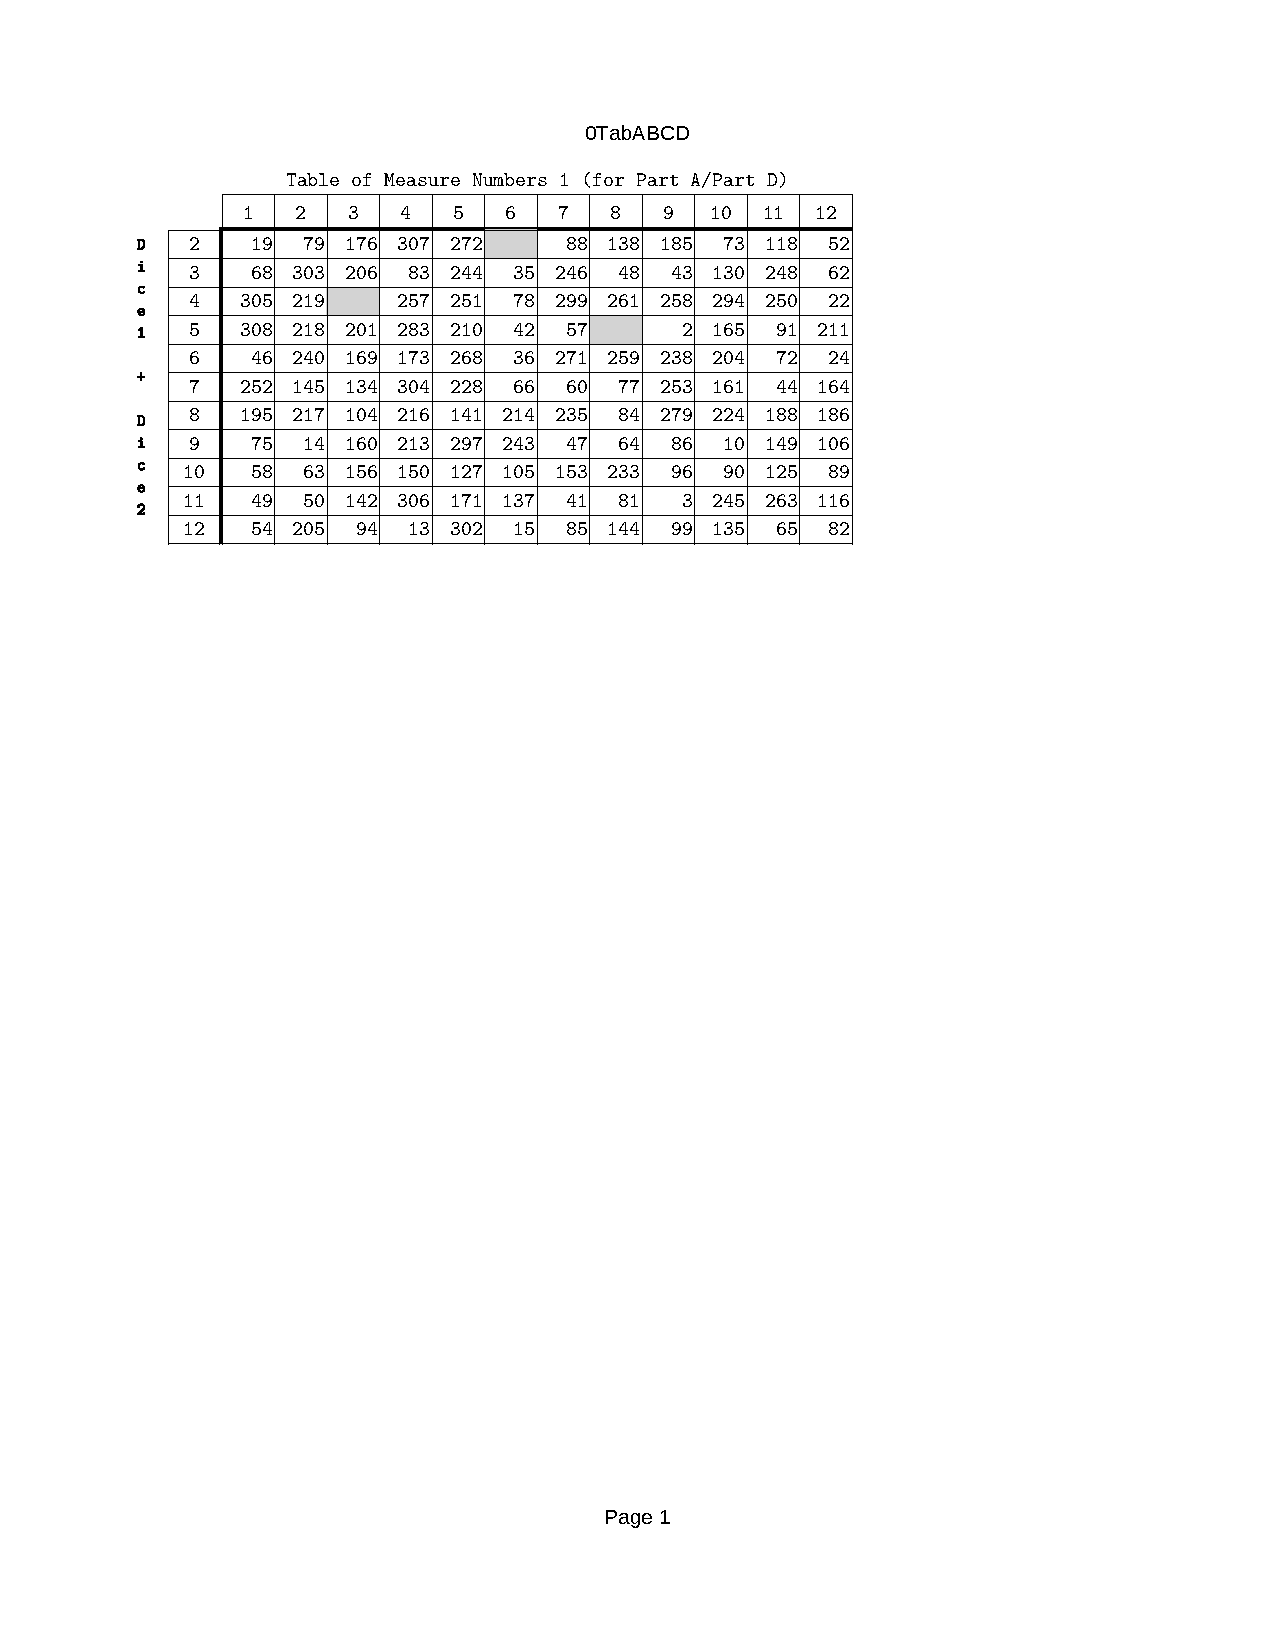
\includegraphics[clip=true,trim=0.75in 7.30in 2.50in 1.10in,scale=0.90]{0TAB-AD}
	\end{tabular}
	\caption{This Table of Measure Numbers gives the measure number to be looked-up in the Table of Measures for Arias (see Figures~\ref{fig:meas1} to \ref{fig:meas9} in Section~\ref{tabMeas}) corresponding to each of the two-dice outcome per bar for the eight bars of the first part (Part A) of the rondo and the last four bars of the optional fourth part (Part D).}
	\label{tab:find1}
\end{table}

\begin{table}[H]
	\centering
	\begin{tabular}{c}
		\centering
		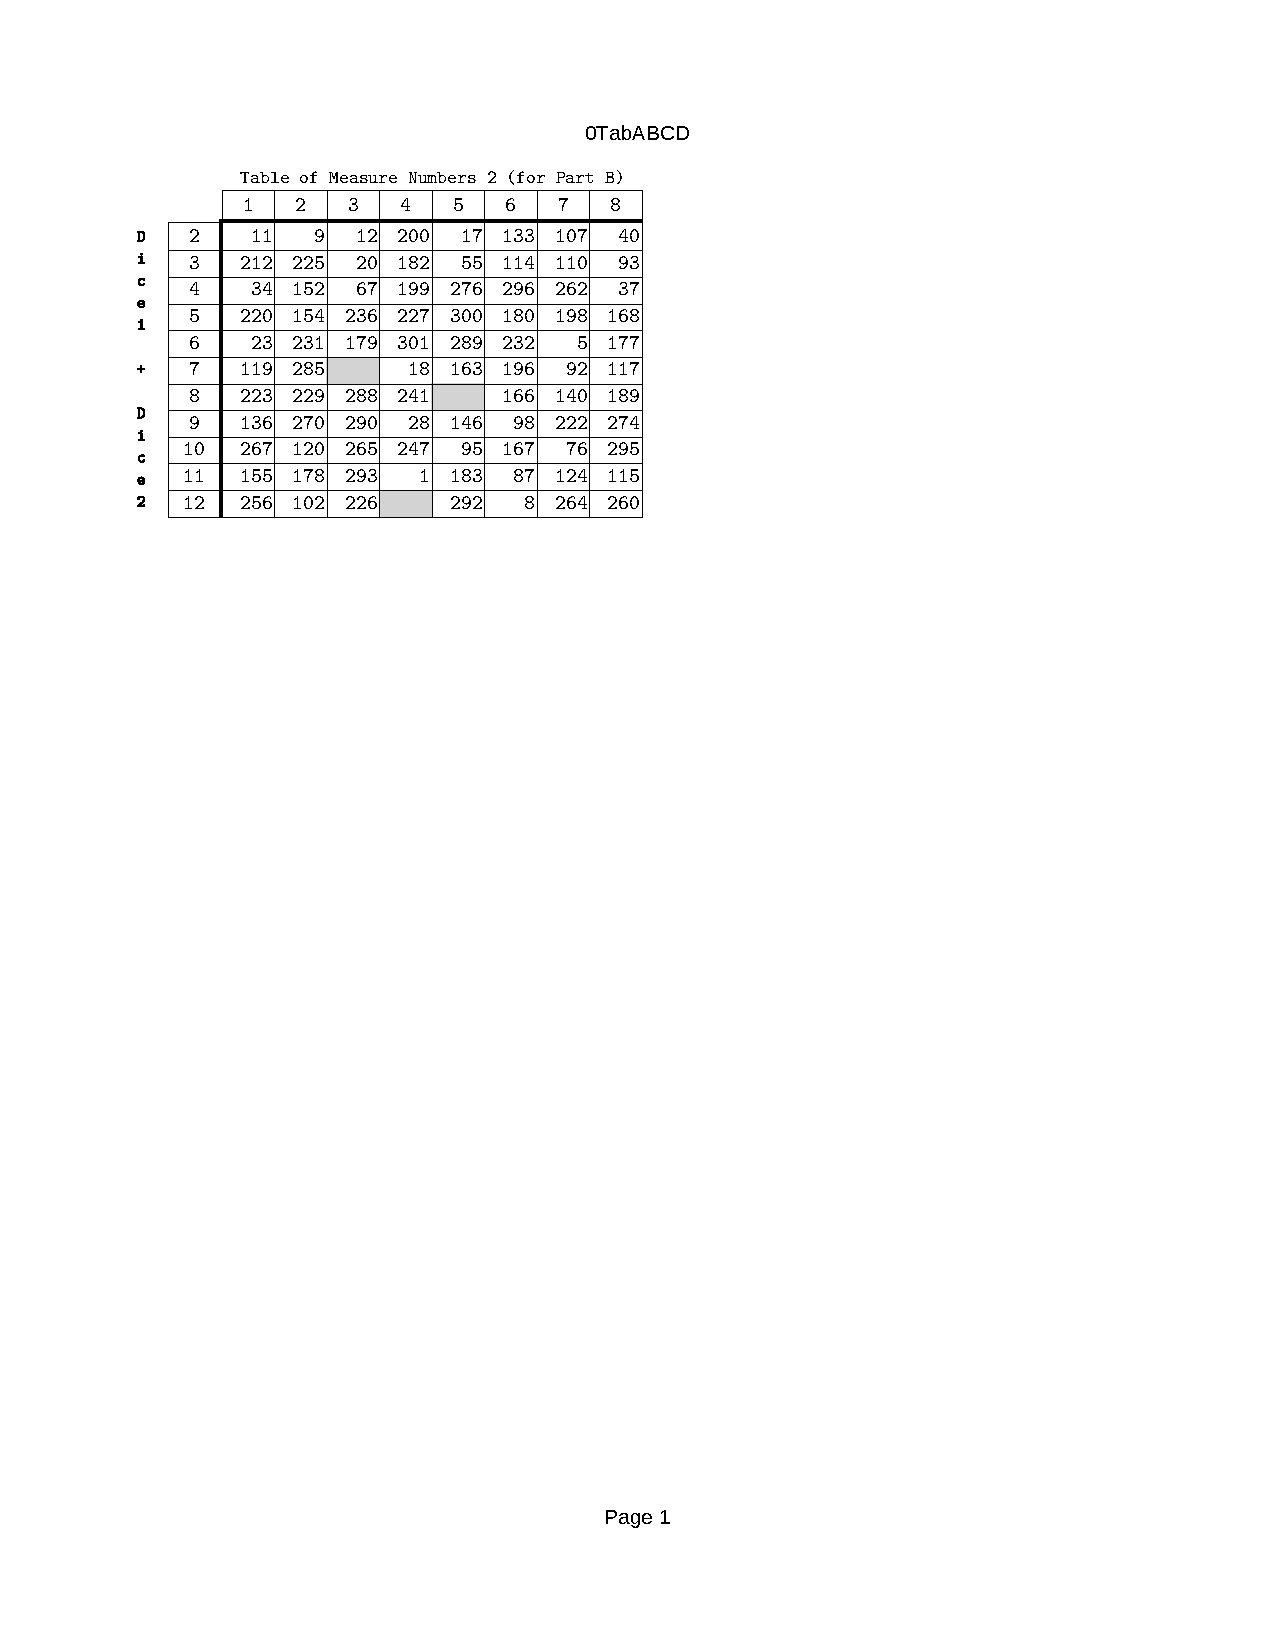
\includegraphics[clip=true,trim=0.75in 7.50in 3.75in 1.10in,scale=0.90]{0TAB-B}
	\end{tabular}
	\caption{This Table of Measure Numbers gives the measure number to be looked-up in the Table of Measures for Arias (see Figures~\ref{fig:meas1} to \ref{fig:meas9} in Section~\ref{tabMeas}) corresponding to each of the two-dice outcome per bar for the eight bars of the second part (Part B) of the rondo.}
	\label{tab:find2}
\end{table}

\begin{table}[H]
	\centering
	\begin{tabular}{c}
		\centering
		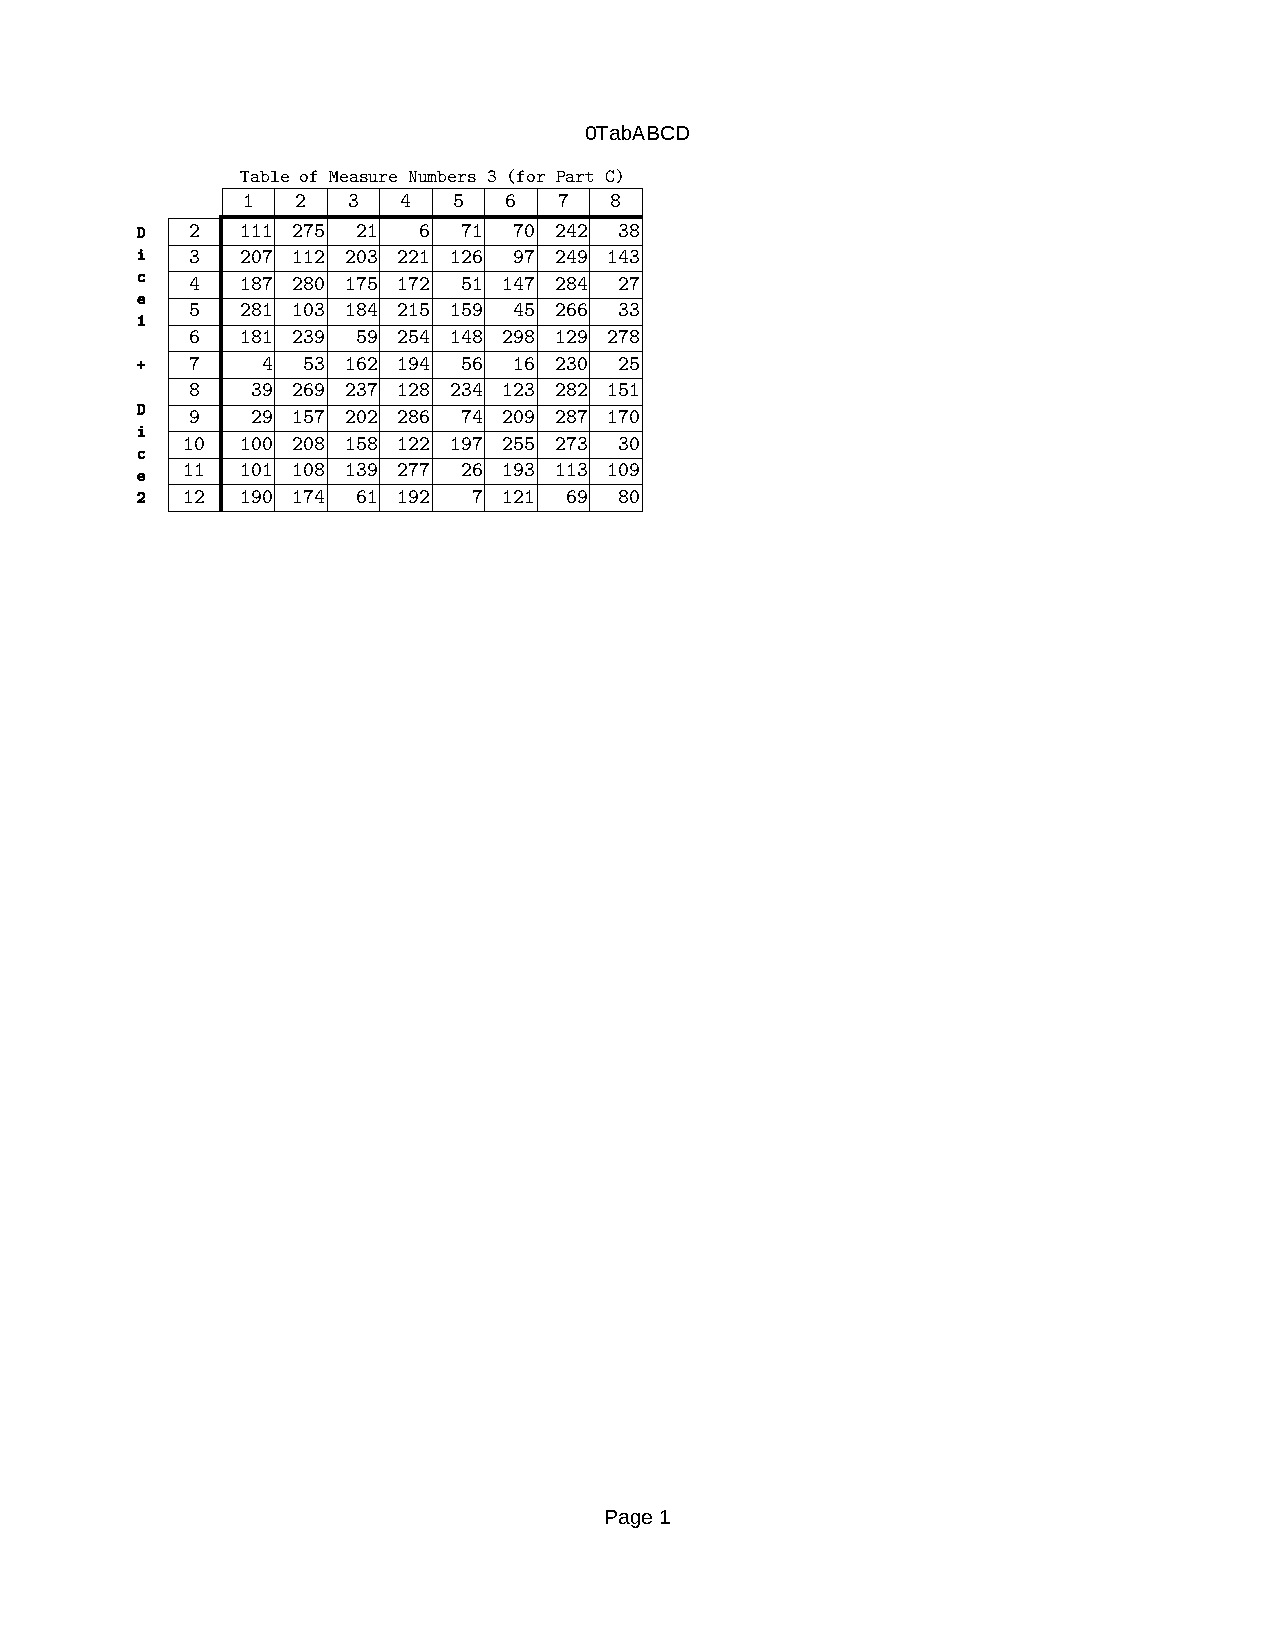
\includegraphics[clip=true,trim=0.75in 7.50in 3.75in 1.10in,scale=0.90]{0TAB-C}
	\end{tabular}
	\caption{This Table of Measure Numbers gives the measure number to be looked-up in the Table of Measures for Arias (see Figures~\ref{fig:meas1} to \ref{fig:meas9} in Section~\ref{tabMeas}) corresponding to each of the two-dice outcome per bar for the eight bars of the second part (Part C) of the rondo.}
	\label{tab:find3}
\end{table}

\begin{table}[H]
	\centering
	\begin{tabular}{c}
		\centering
		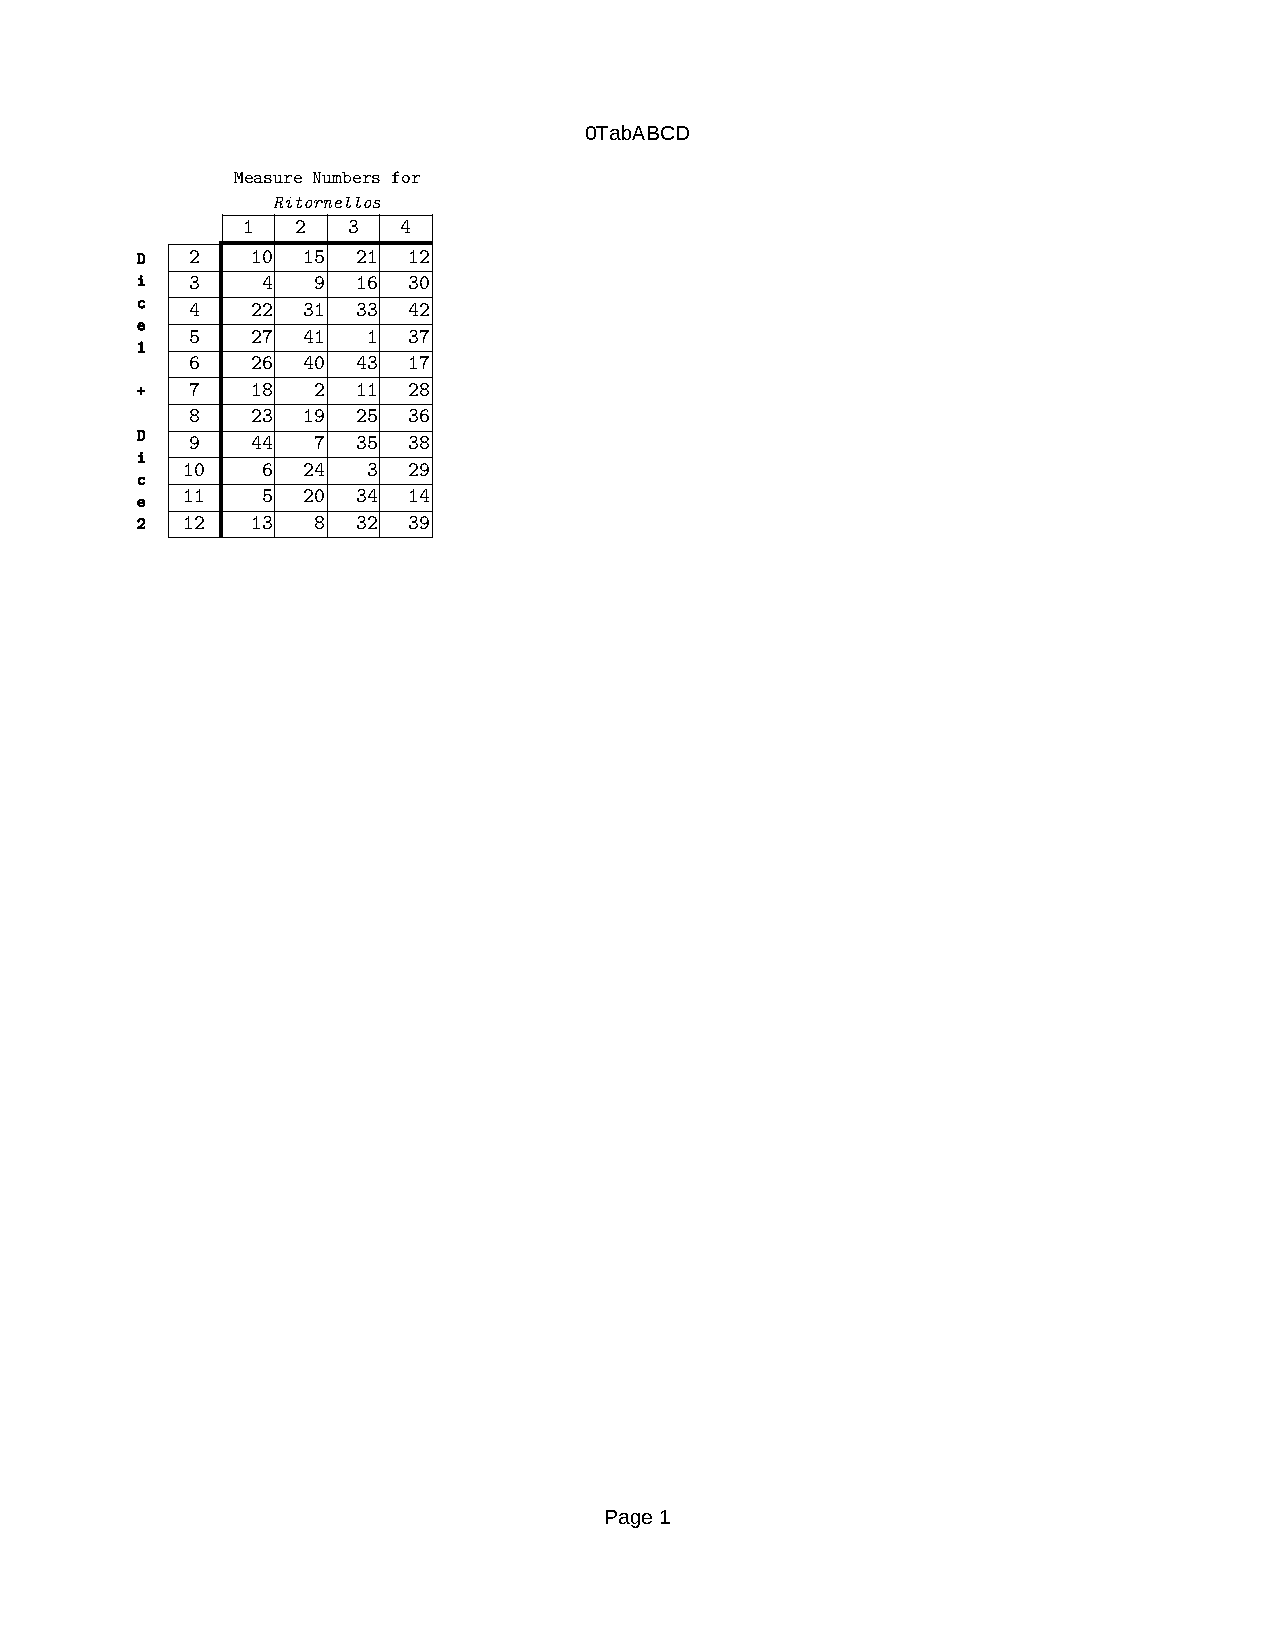
\includegraphics[clip=true,trim=0.75in 7.30in 5.25in 1.00in,scale=0.90]{0TAB-R}
	\end{tabular}
	\caption{This Table of Measure Numbers gives the measure number to be looked-up in the Table of Measures for {\it Ritornellos} (see Figures~\ref{fig:meas10} to \ref{fig:meas12} in Section~\ref{tabMeas}) corresponding to each of the two-dice outcome per bar for the last four bars of the optional fourth part (Part D) of the rondo.}
	\label{tab:find4}
\end{table}


\subsection{Table of Measures}\label{tabMeas}

The Table of Measures for {\em L'Art - 5th Cahier - Ariettas} are given in Figures~\ref{fig:meas1} to \ref{fig:meas9} that follow while the  Table of Measures for {\em L'Art - 5th Cahier - Ritornellos} are given in Figures~\ref{fig:meas10}, \ref{fig:meas11}, and Figures~\ref{fig:meas12}.  These are all based but not exactly identical to those that are given in Antonio Calegaris's \href{https://imslp.org/wiki/L'art\_de_composer\_de\_la_musique\_sans\_en\_conna\%C3\%AEtre\_les\_\%C3\%A9l\%C3\%A9ments\_(Calegari\%2C\_Antonio)}{{\em L'Art - 5th Cahier}}.

%\newpage
${}_{}$\\
\vspace{0.10in}
\addcontentsline{toc}{subsection}{\hspace*{0.25in} {\em L'Art - 5th Cahier - Ariettas} page 1 of measures}	
\begin{figure}[H]
	\centering
	\def\svgwidth{0.975\columnwidth}
	\input{calegari-ariettas001.pdf_tex}
	\caption{Table of Measures - Ariettas (Page 1/9)}
	\label{fig:meas1}
\end{figure}

\newpage
${}_{}$\\
\vspace{0.10in}
\addcontentsline{toc}{subsection}{\hspace*{0.25in} {\em L'Art - 5th Cahier - Ariettas} page 2 of measures}	
\begin{figure}[H]
	\centering
	\def\svgwidth{0.975\columnwidth}
	\input{calegari-ariettas002.pdf_tex}
	\caption{Table of Measures - Ariettas (Page 2/9)}
	\label{fig:meas2}
\end{figure}

\newpage
${}_{}$\\
\vspace{0.10in}
\addcontentsline{toc}{subsection}{\hspace*{0.25in} {\em L'Art - 5th Cahier - Ariettas} page 3 of measures}	
\begin{figure}[H]
	\centering
	\def\svgwidth{0.975\columnwidth}
	\input{calegari-ariettas003.pdf_tex}
\caption{Table of Measures - Ariettas (Page 3/9)}
	\label{fig:meas3}
\end{figure}

\newpage
${}_{}$\\
\vspace{0.10in}
\addcontentsline{toc}{subsection}{\hspace*{0.25in} {\em L'Art - 5th Cahier - Ariettas} page 4 of measures}	
\begin{figure}[H]
	\centering
	\def\svgwidth{0.975\columnwidth}
	\input{calegari-ariettas004.pdf_tex}
\caption{Table of Measures - Ariettas (Page 4/9)}
	\label{fig:meas4}
\end{figure}

\newpage
${}_{}$\\
\vspace{0.10in}
\addcontentsline{toc}{subsection}{\hspace*{0.25in} {\em L'Art - 5th Cahier - Ariettas} page 5 of measures}	
\begin{figure}[H]
	\centering
	\def\svgwidth{0.975\columnwidth}
	\input{calegari-ariettas005.pdf_tex}
	\caption{Table of Measures - Ariettas (Page 5/9)}
	\label{fig:meas5}
\end{figure}

\newpage
${}_{}$\\
\vspace{0.10in}
\addcontentsline{toc}{subsection}{\hspace*{0.25in} {\em L'Art - 5th Cahier - Ariettas} page 6 of measures}	
\begin{figure}[H]
	\centering
	\def\svgwidth{0.975\columnwidth}
	\input{calegari-ariettas006.pdf_tex}
	\caption{Table of Measures - Ariettas (Page 6/9)}
	\label{fig:meas6}
\end{figure}

\newpage
${}_{}$\\
\vspace{0.10in}
\addcontentsline{toc}{subsection}{\hspace*{0.25in} {\em L'Art - 5th Cahier - Ariettas} page 7 of measures}	
\begin{figure}[H]
	\centering
	\def\svgwidth{0.975\columnwidth}
	\input{calegari-ariettas007.pdf_tex}
	\caption{Table of Measures - Ariettas (Page 7/9)}
	\label{fig:meas7}
\end{figure}

\newpage
${}_{}$\\
\vspace{0.10in}
\addcontentsline{toc}{subsection}{\hspace*{0.25in} {\em L'Art - 5th Cahier - Ariettas} page 8 of measures}	
\begin{figure}[H]
	\centering
	\def\svgwidth{0.975\columnwidth}
	\input{calegari-ariettas008.pdf_tex}
	\caption{Table of Measures - Ariettas (Page 8/9)}
	\label{fig:meas8}
\end{figure}

\newpage
${}_{}$\\
\vspace{0.10in}
\addcontentsline{toc}{subsection}{\hspace*{0.25in} {\em L'Art - 5th Cahier - Ariettas} page 9 of measures}	
\begin{figure}[H]
	\centering
	\def\svgwidth{0.975\columnwidth}
	\input{calegari-ariettas009.pdf_tex}
	\caption{Table of Measures - Ariettas (Page 9/9)}
	\label{fig:meas9}
\end{figure}

\newpage
${}_{}$\\
\vspace{0.10in}
\addcontentsline{toc}{subsection}{\hspace*{0.25in} {\em L'Art - 5th Cahier - Ritornellos} page 1 of measures}	
\begin{figure}[H]
	\centering
	\def\svgwidth{0.975\columnwidth}
	\input{calegari-ritornellos001.pdf_tex}
	\caption{Table of Measures - Ritornellos (Page 1/3)}
	\label{fig:meas10}
\end{figure}

\newpage
${}_{}$\\
\vspace{0.10in}
\addcontentsline{toc}{subsection}{\hspace*{0.25in} {\em L'Art - 5th Cahier - Ritornellos} page 2 of measures}	
\begin{figure}[H]
	\centering
	\def\svgwidth{0.975\columnwidth}
	\input{calegari-ritornellos002.pdf_tex}
	\caption{Table of Measures - Ritornellos (Page 2/3)}
	\label{fig:meas11}
\end{figure}

\newpage
${}_{}$\\
\vspace{0.10in}
\addcontentsline{toc}{subsection}{\hspace*{0.25in} {\em L'Art - 5th Cahier - Ritornellos} page 3 of measures}	
\begin{figure}[H]
	\centering
	\def\svgwidth{0.975\columnwidth}
	\input{calegari-ritornellos003.pdf_tex}
	\caption{Table of Measures - Ritornellos (Page 3/3)}
	\label{fig:meas12}
\end{figure}


%\newpage
\section{Related Links}
The following are very interesting sites in that they allow the online rendering of MDGs:
\begin{itemize}
	\item \href{https://opus-infinity.org}{Opus Infinity} - Collaborative work of Robbert Harms, Hein Moors, and Suus van Petegem whose goal is to unravel the mystery behind the tables used for generating MDGs.  Site visitors can generate MDGs based on works of Kirnberger, Mozart, Stadler/Haydn, Bach, Gerlach, and Callegari ({\it 1st Cahier}).  Corresponding audio files ({\tt mid, ogg,} and/or {\tt mp3}) and image files ({\tt pdf} or {\tt png}) are also made available for listening, viewing, or downloading.
	
	\item  \href{http://sunsite.univie.ac.at/Mozart/dice/}{Mozart} - A site maintained by John Chuang that allows the site visitor to generate MDGs based on the work of Stadler/Haydn.
	
	\item  \href{https://marian-aldenhoevel.de/mozart/}{Mozart} - A site maintained by Marian Aldenh\"{o}vel allows the visitor to generate a MDG (user-specified or randomly-generated) and the corresponding audio ({\tt midi, wav}) and image files ({\tt pdf, png}) based on {\em Musikalisches W\"{u}rferspiel, K.\ 516f}.
	
	\item \href{https://www.amaranthpublishing.com/mozart.zip}{\tt mozart.zip} -  This is a Windows software ({\small\textcopyright} 1995 VisionSoft) by John Chuang and Stephen Goodwin that generates MDG based on input from user and is available for {\it free} from  \href{http://www.amaranthpublishing.com/MozartDiceGame.htm}{Amaranth Publishing}.  
	
	\item \href{(http://www.asahi-net.or.jp/\~rb5h-ngc/e/k516f.htm}{``Mozart - Musical Game in C K. 516f,"}	Mozart Studies Online - The site of Hideo Noguchi that offers an explanation linking {\em Musikalisches W\"{u}rferspiel, K.\ 516f}, and  {\em K.\ 294d (K.\ Anh.\ C 30.01)}. 
\end{itemize}

\newpage
\section{Acknowledgments}
Special thanks to \href{https://imslp.org}{International Music Score Library Project} for \href{https://imslp.org/wiki/L'art\_de_composer\_de\_la_musique\_sans\_en\_conna\%C3\%AEtre\_les\_\%C3\%A9l\%C3\%A9ments\_(Calegari\%2C\_Antonio)}{\it L'art de composer de la musique sans en connaître les éléments  2nd Ed. (1802)}, \href{https://opus-infinity.org}{Opus Infinity} for additional related information, and \href{http://www.amaranthpublishing.com/MozartDiceGame.htm}{Amaranth Publishing} for a copy of {\tt mozart.zip}. My sincerest gratitude to Chris Walshaw et al. for the \href{http://www.abcnotation.com/}{ABC music notation}; Jean-Francois Moine for \href{http://moinejf.free.fr/}{\tt abcm2ps} and the accompanying examples, templates, and pointers for the appropriate use of these resources; Guido Gonzato for the \href{http://abcplus.sourceforge.net/}{ABC Plus Project} and the \href{http://abcplus.sourceforge.net/#abcMIDI}{{\tt abcmidi} resources} available there, more especially for the ABC resource book {\em Making Music with ABC 2}; James R. Allwright and Seymour Shlien for \href{http://abc.sourceforge.net/abcMIDI}{\tt abcmidi} source and binaries; \href{https://artifex.com/}{Artifex, Inc.} for Ghostscript v.10.00.0 (includes the {\tt ps2pdf} converter); \href{https://www.inkscape.org/}{Inkscape v.1.2.2} for the tool for converting SVGs to PDFs for inclusion into \LaTeX\ documents; William Schelter for \href{https://maxima.sourceforge.io}{Maxima v.5.47.0}---used for computing the permutation number; \href{https://google.lens}{Google Lens} and \href{https://translate.google.com}{Google Translate} for aiding in producing the English versions of the text of {\it L'Art - 5th Cahier}; Colomban Wendling et.\ al for \href{https://www.geany.org}{Geany 2.0 IDE}; and \href{https://tex.stackexchange.com/users/632/martin-h}{\tt User:Martin H} for his \href{https://tex.stackexchange.com/questions/2099/how-to-include-svg-diagrams-in-latex}{reply} to a \TeX\ / \LaTeX\ Stack Exchange question on including SVGs into \LaTeX\ documents. Thanks to  Ditto to Machtelt Garrels for the book \href{http://tldp.org/LDP/Bash-Beginners-Guide/html/Bash-Beginners-Guide.html}{Bash Guide for Beginners}, Vivek Gite for the book \href{http://www.freeos.com/guides/lsst/}{Linux Script Shell Tutorial}, and Steve Parker for the \href{http://steve-parker.org/sh/cheatsheet.pdf}{Unix/Linux Shell Cheatsheet}. John Fogarty's GitHub Site: \href{https://github.com/jfogarty/latex-createspace-bookcover}{Latex CreateSpace BookCover} and Peter Wilson's reply in  \TeX\ / \LaTeX\ Stack Exchange on \href{https://tex.stackexchange.com/questions/17579/how-can-i-design-a-book-cover}{designing a book cover}, were sources of ideas, information, and materials for creating the book cover and title page, thanks to both of them; \href{http://www.libreoffice.org/}{LibreOffice Calc} for its use in the image creation of the book cover.  Many thanks, too, to the \href{https://www.debian.org}{Debian Project} for the Debian 12 (Bookworm) GNU/Linux OS, \href{http://www.tug.org/texlive/}{TeXLive} for providing the \TeX\ distribution,  and \href{https://github.com}{GitHub} for its generosity in providing space for \href{https://github.com/justineuro/mdgBookSVG6Kit}{the project}.  

%\newpage
\section{Twenty (20) Selected Rondos based on {\it L'Art - 5th Cahier}}
%\vspace{-.10in}
This section contains an example of 20 rondos that were generated using the Rules in Section~\ref{mdgRules}.  As mentioned above in Step 6 of the Rules (see Section~\ref{mdgRules}), the parts are played as {\tt (AR)2}.{\tt(BAR)2}.{\tt (CAR)2}.{\tt (BDAR)2} or  {\tt AR}.{\tt AR}.{\tt BAR}.{\tt BAR}.{\tt CAR}.{\tt CAR}.{\tt BDAR}.{\tt BDAR} and that there are a total number of either 74, 75, or 76 bars; when played with repeats, a total of 148, 150, or 152 bars are played for each rondo.
\vspace{-.10in}

{
\topmargin -0.25in
\textheight 9.25in
\input{svgList}
}	

\newpage
\vspace{0.25in}
\section{License}
This work by I Am The Author, based on work of J.L.A. Uro at  \url{https://github.com/justineuro/mdgBookSVG7Kit}, is licensed under a Creative Commons Public Domain International License.

\bibliographystyle{plainnat}
\bibliography{mdg7}

 

\end{document}
